\paragraph{Cấu hình đã sinh ra số công bố.} Nhật ký huấn luyện ghi, ở mỗi epoch, giá trị trung bình của loss đơn điệu. Trong bản mã tải lên cùng bài báo, loss này là $\sum \operatorname{ReLU}(y_2 - y_1)$, chỉ tính từ nhãn của hai chu kỳ liền nhau. Ở cả 39 nhóm, giá trị ghi trong nhật ký là một hằng số qua mọi epoch của cả mười lần chạy, và ở cả 39 nhóm hằng số đó bằng đúng biểu thức trên tính trên các hàng train mà lớp đọc dữ liệu của bài tạo ra từ dữ liệu ở đây (ví dụ 0{,}043214 ở batch 2C của XJTU). Số hạng này vì vậy chỉ cộng thêm một hằng số và không có gradient: số liệu công bố đến từ mô hình chỉ học với loss dữ liệu và loss PDE. Sự trùng khớp này cũng cho thấy cách chia dựng lại và dữ liệu ở đây cho đúng các hàng train của mọi nhóm công bố. Hai bản sửa sau đó đổi số hạng thành $\sum \operatorname{ReLU}(u_2 - u_1)$ rồi $\sum \operatorname{ReLU}\big((u_2 - u_1)(y_1 - y_2)\big)$, và ghi chú mới nhất của kho mã cho biết trọng số $\alpha, \beta$ đã đổi sau khi sửa lỗi; trọng số mặc định trong các script hiện tại không còn khớp với nhật ký.

\paragraph{Chạy lại.} Bảng~\ref{tab:bench} và Hình~\ref{fig:bench} cho kết quả. Bản đã sinh số công bố, chạy 10 lần mỗi nhóm với siêu tham số trong nhật ký, cho sai số bằng 1{,}04--1{,}19 lần số công bố ở bốn bộ đầy đủ và 0{,}97--1{,}20 lần ở chế độ ít mẫu. So theo từng cell test, bản chạy lại cao hơn số công bố có ý nghĩa ở 2 trên 4 bộ đầy đủ. Độ lệch chuẩn giữa các lần chạy bằng 4--34\,\% giá trị trung bình, nên các lần chạy đơn lẻ chênh nhau cỡ khoảng cách trên. Các hàng train trùng khớp, nên phần chênh còn lại đến từ phần cứng, phiên bản thư viện và hạt giống; đồ án không dựng lại được môi trường gốc nên không biết yếu tố nào gây ra phần chênh có hệ thống. Vì vậy báo cáo nêu cả số công bố lẫn số chạy lại, và dùng số chạy lại cho kiểm định ghép cặp vì có dự đoán theo từng cell trong điều kiện đã biết. Bản hiện tại của mã (3 lần mỗi nhóm) cho sai số bằng 0{,}93--1{,}02 lần bản công bố ở bốn bộ đầy đủ và ở chế độ ít mẫu của HUST (không trường hợp nào trong 8 khác có ý nghĩa), nhưng 1{,}54--1{,}87 lần ở chế độ ít mẫu của XJTU với $K \ge 2$ (cao hơn có ý nghĩa ở 2 trên 3), nơi script hiện tại vẫn đặt $\beta = 10$ cho loss đơn điệu nay đã có tác dụng.

\begin{table}[!htbp]\centering\small\setlength{\tabcolsep}{4pt}
\caption[So với PINN4SOH trên đúng cách chia của bài]{MAE theo cell ($\times10^{-3}$) trên đúng các nhóm của PINN4SOH, trung bình qua cell test, lần chạy và nhóm như bài. Chạy lại: mã gốc ở bản đã sinh số công bố (siêu tham số theo nhật ký, 10 lần chạy mỗi nhóm) và ở bản hiện tại (loss đơn điệu đã sửa, trọng số mặc định mới, 3 lần chạy); $\pm$ là độ lệch chuẩn qua lần chạy. Mô hình của đồ án: 3 hạt giống. $K$: số cell có nhãn trong thí nghiệm ít mẫu. $^{*}$/$^{\dagger}$: PINN-lai với tiền xử lý của bài thấp hơn/cao hơn có ý nghĩa so với mã gốc chạy lại bản công bố (Wilcoxon theo cell test, Holm qua 12 hàng).}\label{tab:bench}
\begin{adjustbox}{max width=\textwidth}\begin{tabular}{llrrrrrr}\toprule
 & & \multicolumn{3}{c}{PINN4SOH} & \multicolumn{2}{c}{tiền xử lý của bài} & không rò rỉ \\\cmidrule(lr){3-5}\cmidrule(lr){6-7}\cmidrule(lr){8-8}
Bộ & Chế độ & công bố & chạy lại, bản công bố & chạy lại, bản đã sửa & PINN-lai & GBDT & PINN-lai \\\midrule
XJTU & đầy đủ & 7{,}85 & 8{,}66 $\pm$ 1{,}04 & 8{,}08 $\pm$ 0{,}26 & 6{,}62 & 6{,}82 & 7{,}81 \\
TJU & đầy đủ & 9{,}79 & 11{,}21 $\pm$ 0{,}47 & 10{,}87 $\pm$ 0{,}22 & 8{,}78$^{*}$ & 8{,}63 & 6{,}16 \\
MIT & đầy đủ & 6{,}18 & 7{,}36 $\pm$ 0{,}69 & 7{,}48 $\pm$ 0{,}97 & 6{,}80 & 6{,}15 & 1{,}43 \\
HUST & đầy đủ & 7{,}57 & 7{,}90 $\pm$ 0{,}80 & 7{,}38 $\pm$ 0{,}37 & 6{,}45$^{*}$ & 6{,}16 & 12{,}51 \\
\addlinespace
XJTU & $K = 1$ & 31{,}54 & 30{,}70 $\pm$ 8{,}47 & 27{,}09 $\pm$ 8{,}35 & 10{,}51$^{*}$ & 10{,}20 & 13{,}27 \\
 & $K = 2$ & 10{,}06 & 11{,}54 $\pm$ 1{,}34 & 17{,}77 $\pm$ 0{,}99 & 7{,}72 & 8{,}22 & 13{,}60 \\
 & $K = 3$ & 7{,}98 & 9{,}24 $\pm$ 1{,}13 & 16{,}44 $\pm$ 0{,}27 & 7{,}15 & 7{,}04 & 9{,}48 \\
 & $K = 4$ & 7{,}62 & 9{,}17 $\pm$ 1{,}09 & 17{,}18 $\pm$ 0{,}53 & 7{,}20 & 7{,}04 & 8{,}39 \\
\addlinespace
HUST & $K = 1$ & 39{,}42 & 47{,}13 $\pm$ 15{,}83 & 48{,}28 $\pm$ 14{,}94 & 14{,}71$^{*}$ & 10{,}08 & 46{,}72 \\
 & $K = 2$ & 16{,}94 & 18{,}07 $\pm$ 3{,}15 & 16{,}77 $\pm$ 2{,}56 & 11{,}53$^{*}$ & 9{,}66 & 23{,}82 \\
 & $K = 3$ & 14{,}59 & 15{,}10 $\pm$ 1{,}41 & 14{,}68 $\pm$ 1{,}10 & 9{,}16$^{*}$ & 7{,}73 & 21{,}13 \\
 & $K = 4$ & 13{,}62 & 14{,}71 $\pm$ 0{,}60 & 14{,}48 $\pm$ 1{,}09 & 9{,}91$^{*}$ & 8{,}58 & 22{,}64 \\
\bottomrule\end{tabular}\end{adjustbox}\end{table}

\begin{figure}[!htbp]\centering
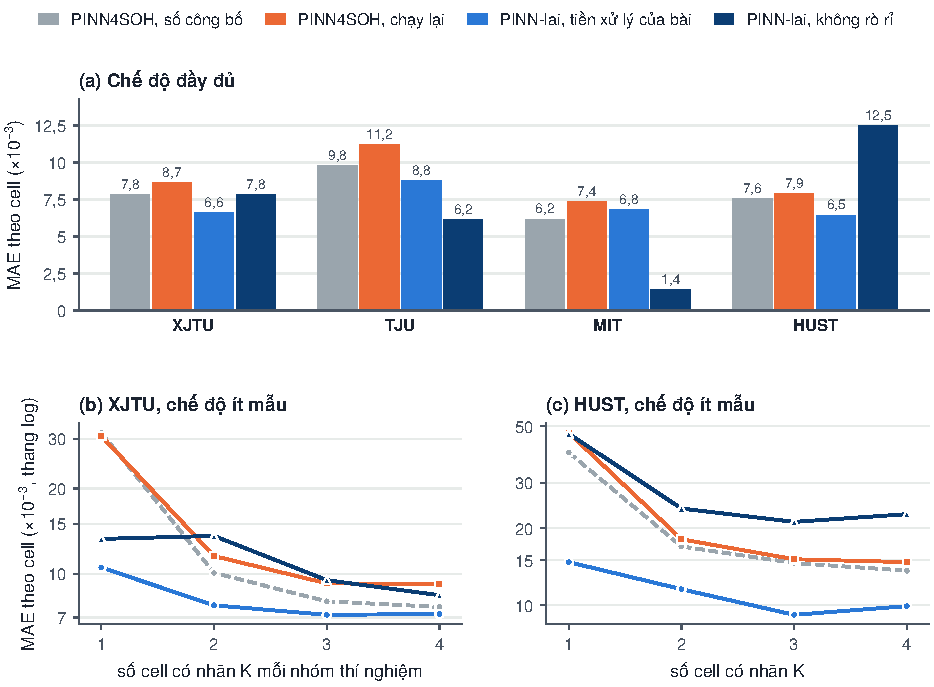
\includegraphics[width=\textwidth]{graphics/fig_benchmark.pdf}
\caption[So với PINN4SOH trên đúng cách chia của bài]{So với PINN4SOH trên đúng cách chia của bài. Trên: chế độ đầy đủ, mỗi bộ năm cột (số công bố, hai bản mã gốc chạy lại với độ lệch chuẩn qua lần chạy, PINN-lai với tiền xử lý của bài và với tiền xử lý không rò rỉ). Dưới: chế độ ít mẫu, MAE theo số cell có nhãn (thang log).}\label{fig:bench}
\end{figure}
